
%%%%%%%%%%%%%%%%%% PREAMBULE %%%%%%%%%%%%%%%%%%

\documentclass[aspectratio=169,utf8]{beamer}
%\documentclass[aspectratio=169,handout]{beamer}

\usetheme{Boadilla}
%\usecolortheme{seahorse}
\usecolortheme[RGB={245,66,24}]{structure}
\useoutertheme{infolines}

% packages
\usepackage{amsfonts,amsmath,amssymb,amsthm}
\usepackage[utf8]{inputenc}
\usepackage[T1]{fontenc}
\usepackage{lmodern}

\usepackage[francais]{babel}
\usepackage{fancybox}
\usepackage{graphicx}

\usepackage{float}
\usepackage{xfrac}

%\usepackage[usenames, x11names]{xcolor}
\usepackage{tikz}
\usepackage{pgfplots}
\usepackage{datetime}



%-----  Package unités -----
\usepackage{siunitx}
\sisetup{locale = FR,detect-all,per-mode = symbol}

%\usepackage{mathptmx}
%\usepackage{fouriernc}
%\usepackage{newcent}
%\usepackage[mathcal,mathbf]{euler}

%\usepackage{palatino}
%\usepackage{newcent}
% \usepackage[mathcal,mathbf]{euler}



% \usepackage{hyperref}
% \hypersetup{colorlinks=true, linkcolor=blue, urlcolor=blue,
% pdftitle={Exo7 - Exercices de mathématiques}, pdfauthor={Exo7}}


%section
% \usepackage{sectsty}
% \allsectionsfont{\bf}
%\sectionfont{\color{Tomato3}\upshape\selectfont}
%\subsectionfont{\color{Tomato4}\upshape\selectfont}

%----- Ensembles : entiers, reels, complexes -----
\newcommand{\Nn}{\mathbb{N}} \newcommand{\N}{\mathbb{N}}
\newcommand{\Zz}{\mathbb{Z}} \newcommand{\Z}{\mathbb{Z}}
\newcommand{\Qq}{\mathbb{Q}} \newcommand{\Q}{\mathbb{Q}}
\newcommand{\Rr}{\mathbb{R}} \newcommand{\R}{\mathbb{R}}
\newcommand{\Cc}{\mathbb{C}} 
\newcommand{\Kk}{\mathbb{K}} \newcommand{\K}{\mathbb{K}}

%----- Modifications de symboles -----
\renewcommand{\epsilon}{\varepsilon}
\renewcommand{\Re}{\mathop{\text{Re}}\nolimits}
\renewcommand{\Im}{\mathop{\text{Im}}\nolimits}
%\newcommand{\llbracket}{\left[\kern-0.15em\left[}
%\newcommand{\rrbracket}{\right]\kern-0.15em\right]}

\renewcommand{\ge}{\geqslant}
\renewcommand{\geq}{\geqslant}
\renewcommand{\le}{\leqslant}
\renewcommand{\leq}{\leqslant}
\renewcommand{\epsilon}{\varepsilon}

%----- Fonctions usuelles -----
\newcommand{\ch}{\mathop{\text{ch}}\nolimits}
\newcommand{\sh}{\mathop{\text{sh}}\nolimits}
\renewcommand{\tanh}{\mathop{\text{th}}\nolimits}
\newcommand{\cotan}{\mathop{\text{cotan}}\nolimits}
\newcommand{\Arcsin}{\mathop{\text{arcsin}}\nolimits}
\newcommand{\Arccos}{\mathop{\text{arccos}}\nolimits}
\newcommand{\Arctan}{\mathop{\text{arctan}}\nolimits}
\newcommand{\Argsh}{\mathop{\text{argsh}}\nolimits}
\newcommand{\Argch}{\mathop{\text{argch}}\nolimits}
\newcommand{\Argth}{\mathop{\text{argth}}\nolimits}
\newcommand{\pgcd}{\mathop{\text{pgcd}}\nolimits} 


%----- Commandes divers ------
\newcommand{\ii}{\mathrm{i}}
\newcommand{\dd}{\text{d}}
\newcommand{\id}{\mathop{\text{id}}\nolimits}
\newcommand{\Ker}{\mathop{\text{Ker}}\nolimits}
\newcommand{\Card}{\mathop{\text{Card}}\nolimits}
\newcommand{\Vect}{\mathop{\text{Vect}}\nolimits}
\newcommand{\Mat}{\mathop{\text{Mat}}\nolimits}
\newcommand{\rg}{\mathop{\text{rg}}\nolimits}
\newcommand{\tr}{\mathop{\text{tr}}\nolimits}


%----- Structure des exercices ------

\newtheoremstyle{styleexo}% name
{2ex}% Space above
{3ex}% Space below
{}% Body font
{}% Indent amount 1
{\bfseries} % Theorem head font
{}% Punctuation after theorem head
{\newline}% Space after theorem head 2
{}% Theorem head spec (can be left empty, meaning ‘normal’)

%\theoremstyle{styleexo}
\newtheorem{exo}{Exercice}
\newtheorem{ind}{Indications}
\newtheorem{cor}{Correction}


\newcommand{\exercice}[1]{} \newcommand{\finexercice}{}
%\newcommand{\exercice}[1]{{\tiny\texttt{#1}}\vspace{-2ex}} % pour afficher le numero absolu, l'auteur...
\newcommand{\enonce}{\begin{exo}} \newcommand{\finenonce}{\end{exo}}
\newcommand{\indication}{\begin{ind}} \newcommand{\finindication}{\end{ind}}
\newcommand{\correction}{\begin{cor}} \newcommand{\fincorrection}{\end{cor}}

\newcommand{\noindication}{\stepcounter{ind}}
\newcommand{\nocorrection}{\stepcounter{cor}}

\newcommand{\fiche}[1]{} \newcommand{\finfiche}{}
\newcommand{\titre}[1]{\centerline{\large \bf #1}}
\newcommand{\addcommand}[1]{}
\newcommand{\video}[1]{}

% Marge
\newcommand{\mymargin}[1]{\marginpar{{\small #1}}}

\def\noqed{\renewcommand{\qedsymbol}{}}


%----- Presentation ------
\setlength{\parindent}{0cm}

%\newcommand{\ExoSept}{\href{http://exo7.emath.fr}{\textbf{\textsf{Exo7}}}}

\definecolor{myred}{rgb}{0.93,0.26,0}
\definecolor{myorange}{rgb}{0.97,0.58,0}
\definecolor{myyellow}{rgb}{1,0.86,0}

\newcommand{\LogoExoSept}[1]{  % input : echelle
{\usefont{U}{cmss}{bx}{n}
\begin{tikzpicture}[scale=0.1*#1,transform shape]
  \fill[color=myorange] (0,0)--(4,0)--(4,-4)--(0,-4)--cycle;
  \fill[color=myred] (0,0)--(0,3)--(-3,3)--(-3,0)--cycle;
  \fill[color=myyellow] (4,0)--(7,4)--(3,7)--(0,3)--cycle;
  \node[scale=5] at (3.5,3.5) {Exo7};
\end{tikzpicture}}
}


\newcommand{\debutmontitre}{
  \author{} \date{} 
  \thispagestyle{empty}
  \hspace*{-10ex}
  \begin{minipage}{\textwidth}
    \titlepage  
  \vspace*{-2.5cm}
  \begin{center}
    \LogoExoSept{2.5}
  \end{center}
  \end{minipage}

  \vspace*{-0cm}
  
  % Astuce pour que le background ne soit pas discrétisé lors de la conversion pdf -> png
\begin{tikzpicture}
        \fill[opacity=0,green!60!black] (0,0)--++(0,0)--++(0,0)--++(0,0)--cycle; 
\end{tikzpicture}

% toc S'affiche trop tot :
% \tableofcontents[hideallsubsections, pausesections]
}

\newcommand{\finmontitre}{
  \end{frame}
  \setcounter{framenumber}{0}
} % ne marche pas pour une raison obscure

%----- Commandes supplementaires ------

% \usepackage[landscape]{geometry}
% \geometry{top=1cm, bottom=3cm, left=2cm, right=10cm, marginparsep=1cm
% }
% \usepackage[a4paper]{geometry}
% \geometry{top=2cm, bottom=2cm, left=2cm, right=2cm, marginparsep=1cm
% }

%\usepackage{standalone}


% New command Arnaud -- november 2011
\setbeamersize{text margin left=24ex}
% si vous modifier cette valeur il faut aussi
% modifier le decalage du titre pour compenser
% (ex : ici =+10ex, titre =-5ex

\theoremstyle{definition}
%\newtheorem{proposition}{Proposition}
%\newtheorem{exemple}{Exemple}
%\newtheorem{theoreme}{Théorème}
%\newtheorem{lemme}{Lemme}
%\newtheorem{corollaire}{Corollaire}
%\newtheorem*{remarque*}{Remarque}
%\newtheorem*{miniexercice}{Mini-exercices}
%\newtheorem{definition}{Définition}

% Commande tikz
\usetikzlibrary{calc}
\usetikzlibrary{patterns,arrows}
\usetikzlibrary{matrix}
\usetikzlibrary{fadings} 

%definition d'un terme
\newcommand{\defi}[1]{{\color{myorange}\textbf{\emph{#1}}}}
\newcommand{\evidence}[1]{{\color{blue}\textbf{\emph{#1}}}}
\newcommand{\assertion}[1]{\emph{\og#1\fg}}  % pour chapitre logique
%\renewcommand{\contentsname}{Sommaire}
\renewcommand{\contentsname}{}
\setcounter{tocdepth}{2}



%------ Figures ------

\def\myscale{1} % par défaut 
\newcommand{\myfigure}[2]{  % entrée : echelle, fichier figure
\def\myscale{#1}
\begin{center}
\footnotesize
{#2}
\end{center}}


%------ Encadrement ------

\usepackage{fancybox}


\newcommand{\mybox}[1]{
\setlength{\fboxsep}{7pt}
\begin{center}
\shadowbox{#1}
\end{center}}

\newcommand{\myboxinline}[1]{
\setlength{\fboxsep}{5pt}
\raisebox{-10pt}{
\shadowbox{#1}
}
}

%--------------- Commande beamer---------------
\newcommand{\beameronly}[1]{#1} % permet de mettre des pause dans beamer pas dans poly


\setbeamertemplate{navigation symbols}{}
\setbeamertemplate{footline}  % tiré du fichier beamerouterinfolines.sty
{
  \leavevmode%
  \hbox{%
  \begin{beamercolorbox}[wd=.333333\paperwidth,ht=2.25ex,dp=1ex,center]{author in head/foot}%
    % \usebeamerfont{author in head/foot}\insertshortauthor%~~(\insertshortinstitute)
    \usebeamerfont{section in head/foot}{\bf\insertshorttitle}
  \end{beamercolorbox}%
  \begin{beamercolorbox}[wd=.333333\paperwidth,ht=2.25ex,dp=1ex,center]{title in head/foot}%
    \usebeamerfont{section in head/foot}{\bf\insertsectionhead}
  \end{beamercolorbox}%
  \begin{beamercolorbox}[wd=.333333\paperwidth,ht=2.25ex,dp=1ex,right]{date in head/foot}%
    % \usebeamerfont{date in head/foot}\insertshortdate{}\hspace*{2em}
    \insertframenumber{} / \inserttotalframenumber\hspace*{2ex} 
  \end{beamercolorbox}}%
  \vskip0pt%
}


\definecolor{mygrey}{rgb}{0.5,0.5,0.5}
\setlength{\parindent}{0cm}
%\DeclareTextFontCommand{\helvetica}{\fontfamily{phv}\selectfont}

% background beamer
\definecolor{couleurhaut}{rgb}{0.85,0.9,1}  % creme
\definecolor{couleurmilieu}{rgb}{1,1,1}  % vert pale
\definecolor{couleurbas}{rgb}{0.85,0.9,1}  % blanc
\setbeamertemplate{background canvas}[vertical shading]%
[top=couleurhaut,middle=couleurmilieu,midpoint=0.4,bottom=couleurbas] 
%[top=fondtitre!05,bottom=fondtitre!60]



\makeatletter
\setbeamertemplate{theorem begin}
{%
  \begin{\inserttheoremblockenv}
  {%
    \inserttheoremheadfont
    \inserttheoremname
    \inserttheoremnumber
    \ifx\inserttheoremaddition\@empty\else\ (\inserttheoremaddition)\fi%
    \inserttheorempunctuation
  }%
}
\setbeamertemplate{theorem end}{\end{\inserttheoremblockenv}}

\newenvironment{theoreme}[1][]{%
   \setbeamercolor{block title}{fg=structure,bg=structure!40}
   \setbeamercolor{block body}{fg=black,bg=structure!10}
   \begin{block}{{\bf Th\'eor\`eme }#1}
}{%
   \end{block}%
}


\newenvironment{proposition}[1][]{%
   \setbeamercolor{block title}{fg=structure,bg=structure!40}
   \setbeamercolor{block body}{fg=black,bg=structure!10}
   \begin{block}{{\bf Proposition }#1}
}{%
   \end{block}%
}

\newenvironment{corollaire}[1][]{%
   \setbeamercolor{block title}{fg=structure,bg=structure!40}
   \setbeamercolor{block body}{fg=black,bg=structure!10}
   \begin{block}{{\bf Corollaire }#1}
}{%
   \end{block}%
}

\newenvironment{mydefinition}[1][]{%
   \setbeamercolor{block title}{fg=structure,bg=structure!40}
   \setbeamercolor{block body}{fg=black,bg=structure!10}
   \begin{block}{{\bf Définition} #1}
}{%
   \end{block}%
}

\newenvironment{lemme}[0]{%
   \setbeamercolor{block title}{fg=structure,bg=structure!40}
   \setbeamercolor{block body}{fg=black,bg=structure!10}
   \begin{block}{\bf Lemme}
}{%
   \end{block}%
}

\newenvironment{remarque}[1][]{%
   \setbeamercolor{block title}{fg=black,bg=structure!20}
   \setbeamercolor{block body}{fg=black,bg=structure!5}
   \begin{block}{Remarque #1}
}{%
   \end{block}%
}


\newenvironment{exemple}[1][]{%
   \setbeamercolor{block title}{fg=black,bg=structure!20}
   \setbeamercolor{block body}{fg=black,bg=structure!5}
   \begin{block}{{\bf Exemple }#1}
}{%
   \end{block}%
}


\newenvironment{miniexercice}[0]{%
   \setbeamercolor{block title}{fg=structure,bg=structure!20}
   \setbeamercolor{block body}{fg=black,bg=structure!5}
   \begin{block}{Mini-exercices}
}{%
   \end{block}%
}


\newenvironment{tp}[0]{%
   \setbeamercolor{block title}{fg=structure,bg=structure!40}
   \setbeamercolor{block body}{fg=black,bg=structure!10}
   \begin{block}{\bf Travaux pratiques}
}{%
   \end{block}%
}
\newenvironment{exercicecours}[1][]{%
   \setbeamercolor{block title}{fg=structure,bg=structure!40}
   \setbeamercolor{block body}{fg=black,bg=structure!10}
   \begin{block}{{\bf Exercice }#1}
}{%
   \end{block}%
}
\newenvironment{algo}[1][]{%
   \setbeamercolor{block title}{fg=structure,bg=structure!40}
   \setbeamercolor{block body}{fg=black,bg=structure!10}
   \begin{block}{{\bf Algorithme}\hfill{\color{gray}\texttt{#1}}}
}{%
   \end{block}%
}


\setbeamertemplate{proof begin}{
   \setbeamercolor{block title}{fg=black,bg=structure!20}
   \setbeamercolor{block body}{fg=black,bg=structure!5}
   \begin{block}{{\footnotesize Démonstration}}
   \footnotesize
   \smallskip}
\setbeamertemplate{proof end}{%
   \end{block}}
\setbeamertemplate{qed symbol}{\openbox}


\makeatother
\usecolortheme[RGB={192,41,0}]{structure}

% Commande spécifique à ce chapitre
\newcommand{\vect}{\overrightarrow}

\newcommand{\Sage}{\texttt{Sage}}

\usepackage{textcomp}

\usepackage{listings}
\lstset{
  upquote=true,
  columns=flexible,
  keepspaces=true,
  basicstyle=\ttfamily,
  commentstyle=\color{gray},
  language=Python,
  showstringspaces=false,
  aboveskip=0em,  
  belowskip=0em,
  escapeinside=||,
  breaklines=true,
  postbreak=\raisebox{0ex}[0ex][0ex]{\qquad\ensuremath{\color{red}\hookrightarrow\space}},
}

\lstset{
  literate={é}{{\'e}}1
           {è}{{\`e}}1
           {à}{{\`a}}1
}

\newcommand{\codeinline}[1]{\lstinline!#1!}


%%%%%%%%%%%%%%%%%%%%%%%%%%%%%%%%%%%%%%%%%%%%%%%%%%%%%%%%%%%%%
%%%%%%%%%%%%%%%%%%%%%%%%%%%%%%%%%%%%%%%%%%%%%%%%%%%%%%%%%%%%%


\begin{document}
\renewcommand*{\theenumii}{\alph{enumii}}

\title{{\bf Calcul formel}}
\subtitle{Courbes et surfaces (2)}

\begin{frame}
  
  \debutmontitre

  \pause

{\footnotesize
\hfill
\setbeamercovered{transparent=50}
\begin{minipage}{0.6\textwidth}
  \begin{itemize}
    \item<3-> \'Etude d'une courbe paramétrée
    \item<4-> La projection stéréographique
  \end{itemize}
\end{minipage}
}

\end{frame}

\setcounter{framenumber}{0}



%%%%%%%%%%%%%%%%%%%%%%%%%%%%%%%%%%%%%%%%%%%%%%%%%%%%%%%%%%%%%%%%
\section{\'Etude d'une courbe paramétrée}

\begin{frame}
\begin{tp}
\'Etudier en détail la courbe paramétrée du plan définie par 
  $$\left\{
  \begin{array}{l}
  x(t) =  t^3-2t\\[1mm]
  y(t) =  t^2-t
  \end{array}
  \right.\qquad  t \in \Rr.$$
\begin{enumerate}
  \item Tracer la courbe.
  
  \item Trouver les points d'intersection de la courbe avec l'axe des ordonnées.
  
  \item Trouver les points en lesquels la tangente est verticale, puis horizontale.
  
  \item Trouver les coordonnées des points doubles.
\end{enumerate}
\end{tp}
\end{frame}


\begin{frame}
\begin{enumerate} 
  \item ~
\end{enumerate}
\vspace*{-2ex}
\begin{center}
  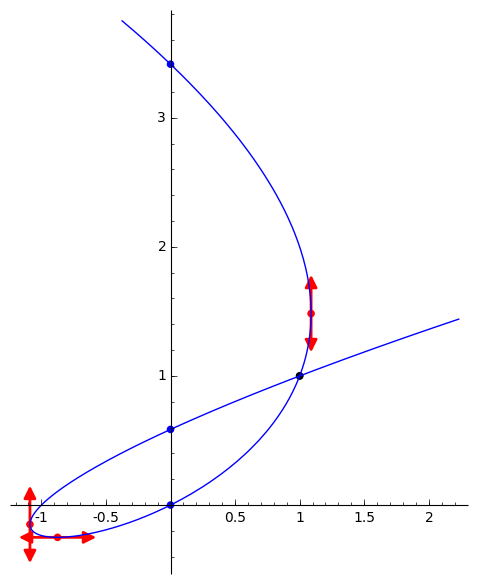
\includegraphics[scale=0.52]{figures/courbe.png} 
\end{center}

\end{frame}


\begin{frame}[fragile]

\begin{enumerate}  
  \setcounter{enumi}{1}
  \item 
  \begin{itemize}
    \item \codeinline{x = t^3-2*t}
    \item \codeinline{y = t^2-t}
    \pause
    \item $x(t)=0$ :  valeurs de $t$ correspondant aux points d'intersection de la courbe avec l'axe $(x=0)$
    \pause
    \item \codeinline{solve(x==0,t)}
    \pause
    \item trois solutions $t \in \{-\sqrt2,0,+\sqrt2\}$
    \pause
    \item trois points
$\{(0,2+\sqrt2),(0,0),(0,2-\sqrt2)\}$
  \end{itemize}

\bigskip
\pause
  
  \item
  \begin{itemize}
    \item \codeinline{xx = diff(x,t)} définit la dérivée $x'(t)$
    
    \item \codeinline{yy = diff(y,t)} définit la dérivée $y'(t)$
    \pause
    \item $x'(t)=0$ : valeurs de $t$ pour lesquelles la tangente à la courbe est verticale
    \pause
    \item \codeinline{solve(xx==0,t)}   
    \pause
    \item \codeinline{solve(yy==0,t)}     
  \end{itemize}    
\end{enumerate}  
\end{frame}


\begin{frame} 
 \begin{enumerate}
  \setcounter{enumi}{3}
  \item
  \begin{itemize}
    \item 
  Trouver les points doubles, c'est résoudre le système :
   $$\left\{
  \begin{array}{l}
  x(s) =  x(t)\\[2mm]
  y(s) =  y(t)
  \end{array}
  \right.\qquad  s,t \in \Rr$$ 
  \pause
    \item Il faut exclure la solution évidente $t=s$
   \pause 
    \item Cela signifie
  que $(s-t)$ divise les polynômes de deux variables $x(s)-x(t)$ et
  $y(s)-y(t)$
  \pause
    \item Le système devient :
   $$\left\{
  \begin{array}{l}
  \dfrac{x(s)-x(t)}{s-t} = 0  \\[3mm]
  \dfrac{y(s)-y(t)}{s-t} = 0
  \end{array}
  \right.\qquad  s,t \in \Rr$$   
  \end{itemize}

\end{enumerate}
\end{frame}


\begin{frame}[fragile]
  %\insertcode{formel/Algos/courbe-tex.sage}{courbe.sage} 
\small
\begin{algo}[courbe.sage]
\begin{lstlisting} 
var('s,t')
x = t^3-2*t
y = t^2-t|\pause|
eqx = x.subs(t=s) - x                    # Equation x(s)-x(t)|\pause|
eqxs = (eqx/(s-t)).simplify_rational()    # (x(s)-x(t))/(s-t)|\pause|
eqy = y.subs(t=s) - y                    # Equation y(s)-y(t)
eqys = (eqy/(s-t)).simplify_rational()    # (y(s)-y(t))/(s-t)|\pause|
points_double = solve([eqxs==0,eqys==0], s,t)     # Solutions
\end{lstlisting}
\end{algo}  

\bigskip
\pause

Fournit la solution 
  $(s,t) = \big(\frac{1-\sqrt5}{2}, \frac{1+\sqrt5}{2}\big)$ : il y a un unique 
  point double ayant pour coordonnées $(1,1)$
\end{frame}


%%%%%%%%%%%%%%%%%%%%%%%%%%%%%%%%%%%%%%%%%%%%%%%%%%%%%%%%%%%%%%%%
\section{La projection stéréographique}

\begin{frame}
\begin{tp}
Soit $ \mathcal{S}$ la sphère centrée à l'origine de $\Rr^3$ et de rayon $1$.
On note $N = (0,0,1)$ le pôle Nord. Soit $\mathcal{P}$ le plan
équatorial d'équation $(z=0)$. La \defi{projection stéréographique}
est l'application $\Phi : \mathcal{S} \setminus \{N\} \to \mathcal{P}$
qui à un point $S$ de la sphère associe le point $P = (NS) \cap \mathcal{P}$
défini par l'intersection de la droite $(NS)$ avec le plan $\mathcal{P}$.

\begin{center}
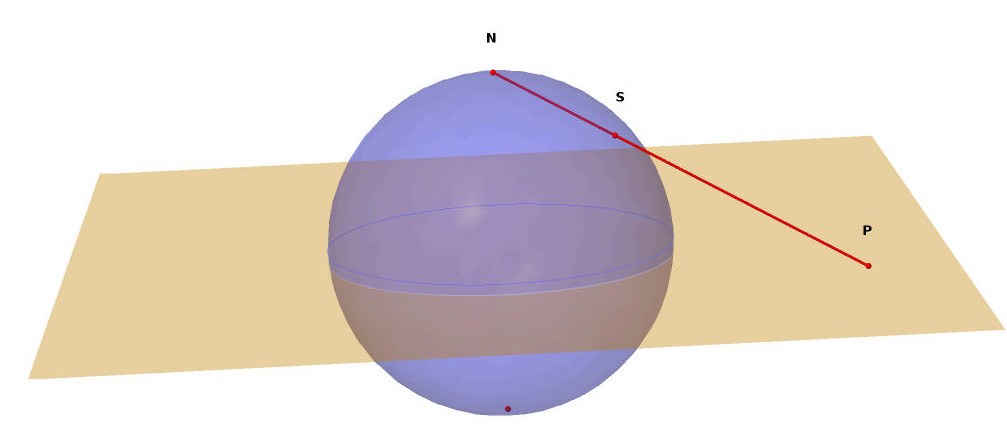
\includegraphics[scale=0.3]{figures/stereo1bis.jpg} 
\end{center}
\end{tp}
\end{frame}


\begin{frame}
\begin{tp}
\begin{enumerate}
  \item En écrivant la relation $\vect{NP} = k \vect{NS}$ et sachant que $P \in \mathcal{P}$, trouver
  $k$ et en déduire $P$.
  
  Vérifier ainsi que l'application $\Phi$ est définie par :
  
  \vspace*{-2ex}
  $$\Phi : \mathcal{S} \setminus \{N\} \to \mathcal{P} \qquad 
  \Phi(x,y,z) = \left( \frac{x}{1-z}, \frac{y}{1-z} \right)$$
  \vspace*{-2ex}
  
  Définir la fonction correspondante avec \Sage.
  
  \item  Définir et vérifier que l'application inverse est $\Psi : \mathcal{P} \to \mathcal{S}\setminus \{N\}$ :
  
  \vspace*{-2ex}
  $$\Psi (X,Y) = \left( \frac{2X}{\rho},\frac{2Y}{\rho},1-\frac{2}{\rho}  \right) \quad \text{ avec } \rho = 1+X^2+Y^2$$
  \vspace*{-2ex}
  
 \end{enumerate}

\end{tp}
\end{frame}


\begin{frame}
\begin{tp}
\begin{enumerate}   
\setcounter{enumi}{2} 
  \item \'Ecrire une fonction qui dessine une courbe paramétrée $\mathcal{C}'$ : $\big( x(t),y(t) \big)$, $t\in[a,b]$
  du plan $\mathcal{P}$, et qui dessine aussi l'image inverse de la courbe sur la sphère, $\mathcal{C} = 
  \Psi(\mathcal{C}')$.
 
  
  \item Vérifier graphiquement deux propriétés fondamentales de la projection stéréographique :
  \begin{enumerate}
    \item \og La projection stéréographique envoie les cercles de la sphère sur des cercles ou des droites du plan.\fg
    \item \og La projection stéréographique préserve les angles.\fg\ En particulier, deux courbes qui se coupent
    à angle droit, s'envoient sur deux courbes qui se coupent à angle droit.
  \end{enumerate}
  
  \item Soit $\mathcal{C}'$ la spirale logarithmique d'équation
  $\big( e^t \cos t, e^t \sin t \big)$, $t \in \Rr$.
  Tracer la loxodromie de la sphère qui est $\mathcal{C} = 
  \Psi(\mathcal{C}')$. 
  
  \item  Soit la courbe $\mathcal{C} \subset \mathcal{S}$
  définie par $\frac{1}{13t^2 - 6t + 2}\big(4t, -6t + 2, 13t^2 - 6t\big)$.
  Montrer que son image $\mathcal{C}' = \Phi(\mathcal{C}) \subset \mathcal{P}$
  est une droite, dont vous déterminerez une équation.
  
\end{enumerate}

\end{tp}
\end{frame}



\begin{frame}[fragile]
\begin{enumerate}
  \item ~

\vspace*{-3ex}
  
\begin{minipage}{0.53\textwidth}
\begin{itemize}
  \item $\vect{NP} = k \vect{NS}$ ($k\in \Rr$)
  
  \uncover<2->{\item en plus $P \in \mathcal{P}$, c-à-d $z_P = 0$}
  \uncover<3->{\item \Sage\ calcule $k = \dfrac{1}{1-z}$}
  \uncover<4->{\item $P = N + k\vect{NS}= \left( \dfrac{x}{1-z}, \dfrac{y}{1-z}, 0 \right)$}
\end{itemize}
\end{minipage} 
\begin{minipage}{0.3\textwidth}
\begin{center}
  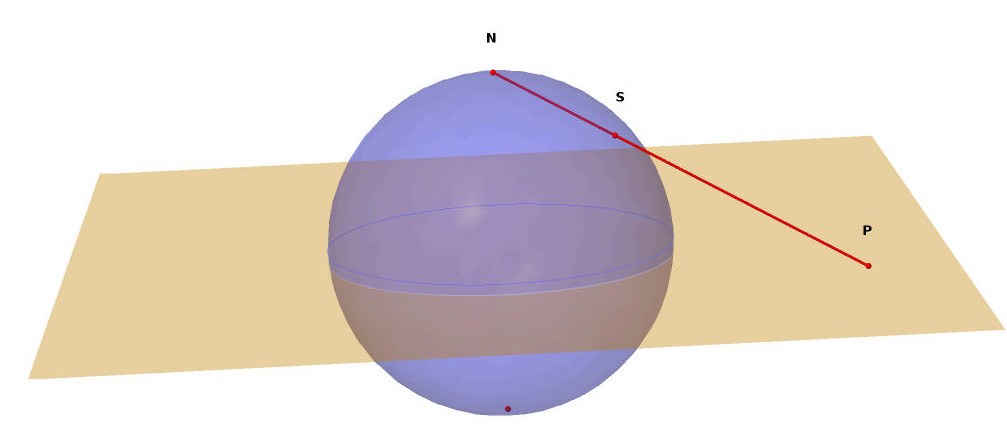
\includegraphics[scale=0.13]{figures/stereo1bis.jpg} 
\end{center}
\end{minipage}  
 
\vspace*{-1ex} 
\pause\pause\pause\pause
 
% \insertcode{formel/Algos/stereographic-tex1.sage}{stereographic.sage (1)} 
\begin{algo}[stereographic.sage (1)]
\begin{lstlisting}  
var('x,y,z,X,Y,k')              
N = vector([0,0,1])    # Points N,S,P comme des vecteurs
S = vector([x,y,z])
P = vector([X,Y,0])
V = (P-N)-k*(S-N)                 # Le vecteur NP - k NS 
eq = V[2]           # On veut troisième coordonnée nulle
sol = solve(eq==0,k)                     # Equation en k
k = sol[0].rhs()                            # Solution k
P = N + k*(S-N)                             # Le point P
\end{lstlisting}
\end{algo} 

\end{enumerate}

\end{frame}  
  
  
  
\begin{frame}[fragile]
\begin{enumerate}
  \item  
  
  $\Phi(x,y,z) = \left( \frac{x}{1-z}, \frac{y}{1-z} \right)$
  
  
%\insertcode{formel/Algos/stereographic-tex2.sage}{stereographic.sage (2)}  
\begin{algo}[stereographic.sage (2)]
\begin{lstlisting}  
def stereo(x,y,z):  
    X = x/(1-z)
    Y = y/(1-z)
    return X,Y
\end{lstlisting}
\end{algo}   


\end{enumerate}

\end{frame}


\begin{frame}[fragile]
\begin{enumerate}
\setcounter{enumi}{1} 
  \item 
  
  $\Psi (X,Y) = \left( \frac{2X}{\rho},\frac{2Y}{\rho},1-\frac{2}{\rho}  \right) \quad \text{ avec } \rho = 1+X^2+Y^2$

%\insertcode{formel/Algos/stereographic-tex3.sage}{stereographic.sage (3)}  
\begin{algo}[stereographic.sage (3)]
\begin{lstlisting}  
def inverse_stereo(X,Y):
    r = 1+X^2+Y^2
    x = 2*X/r
    y = 2*Y/r
    z = 1-2/r
    return x,y,z
\end{lstlisting}
\end{algo}   

\pause
C'est bien la bijection réciproque, c'est-à-dire
  $\Phi\big( \Psi(X,Y) \big) = (X,Y)$ pour tout $(X,Y) \in \Rr^2$ :

\pause
%\insertcode{formel/Algos/stereographic-tex4.sage}{stereographic.sage (4)}
\begin{algo}[stereographic.sage (4)]
\begin{lstlisting}  
newx,newy,newz = inverse_stereo(X,Y)
newX,newY = stereo(newx,newy,newz)
\end{lstlisting}
\end{algo} 

\pause
 et comme \codeinline{newX = X} et \codeinline{newY = Y}, cela prouve le résultat
 
\end{enumerate}
\end{frame}


\begin{frame}[fragile]
\begin{enumerate}
\setcounter{enumi}{2} 
  \item   ~
 %\insertcode{formel/Algos/stereographic-tex5.sage}{stereographic.sage (5)} 

\begin{algo}[stereographic.sage (5)]
\begin{lstlisting} 
def courbes(X,Y,a,b):
    XYtab = [ [X.subs(t=myt),Y.subs(t=myt),0] for myt in srange(a,b,0.1) ]
    xyztab = [ inverse_stereo(coord[0],coord[1]) for coord in XYtab ]
    G = sphere((0,0,0),1)
    G = G + line(XYtab)    
    G = G + line(xyztab)    
   return G
\end{lstlisting}
\end{algo} 

\pause

 Exemple : \codeinline{G = courbes(t^3,t^2,-2,2)}, trace la courbe
 du plan $\big(t^3,t^2\big)$, $t\in[-2,2]$ et son image 
 par la projection stéréographique inverse

\end{enumerate}

\end{frame}


\begin{frame} 

\begin{center}
  \only<1>{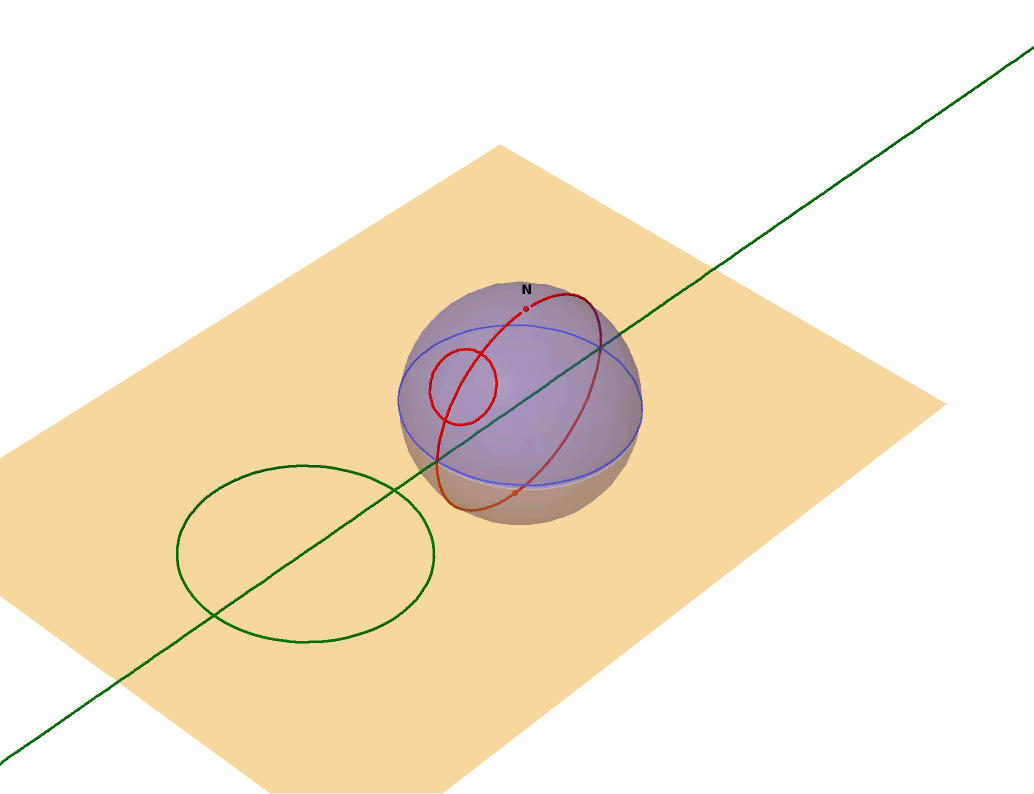
\includegraphics[scale=0.27]{figures/stereo2.jpg}}
  \only<2>{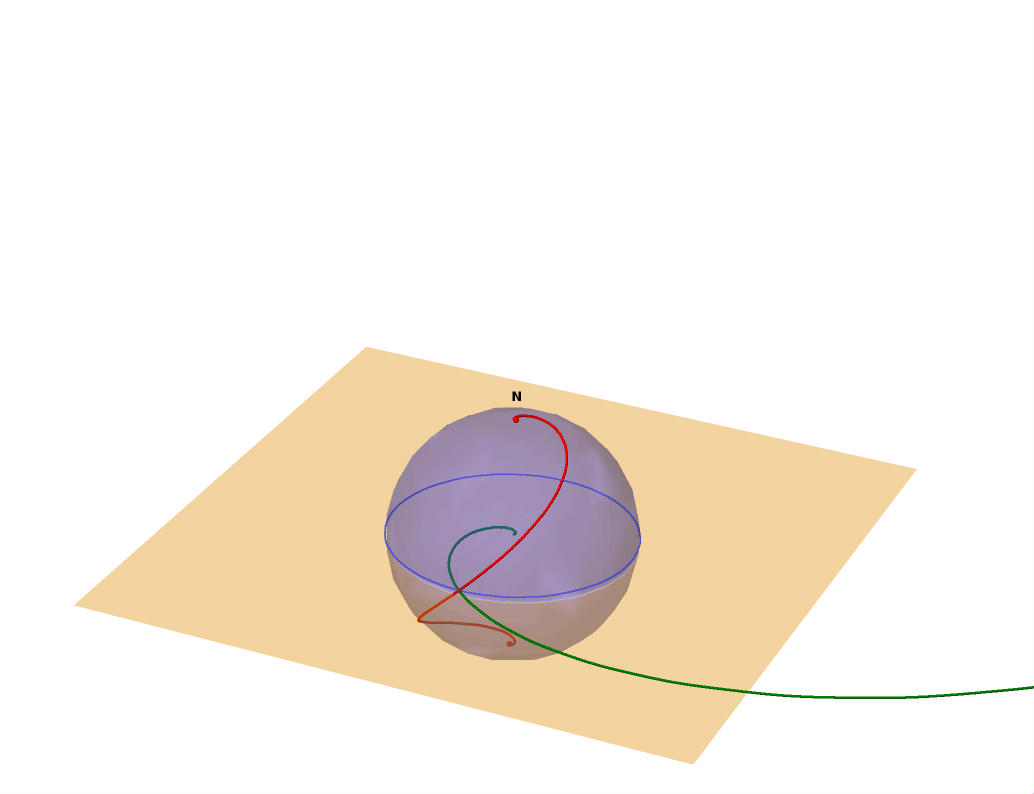
\includegraphics[scale=0.27]{figures/stereo3.jpg}}
\end{center}

\end{frame}

\end{document}

